\documentclass[12pt]{article}

\usepackage{graphicx}
\usepackage{float}
\usepackage{geometry}
\usepackage{amsmath}
\usepackage{microtype}
\usepackage{setspace}
\usepackage{parskip}
\usepackage{booktabs}
\usepackage{multirow}
\usepackage{array}
\usepackage[hidelinks]{hyperref}
\usepackage{tikz}
\usetikzlibrary{shapes,arrows,positioning,fit,backgrounds}

\geometry{margin=1in}
\setstretch{1.15}

\title{AI-Based Predictive Analytics for Diabetes Complications}
\author{
Abdul Wahab \\
Sami Shah \\
Maheer Khurram \\
Sheikh Azan Aziz
}
\date{\today}

\begin{document}

\maketitle
\tableofcontents
\newpage

% ============================================================
% DELIVERABLE 1
% ============================================================

\section*{Deliverable 1: Data Acquisition, Cleaning, and Exploratory Analysis}
\addcontentsline{toc}{section}{Deliverable 1: Data Acquisition, Cleaning, and Exploratory Analysis}

%------------------------------------------------

\section{Introduction}

Diabetes mellitus is a chronic metabolic disorder associated with severe long-term
complications, including kidney disease, neuropathy, and cardiovascular conditions.
Early identification of high-risk patients can improve disease management and reduce
healthcare costs.

This project develops a machine learning-based predictive analytics system to identify
patients at risk of developing multiple diabetes-related complications simultaneously
from clinical data.

%------------------------------------------------

\section{Problem Definition}

Traditional rule-based systems rely on static thresholds and isolated clinical
measurements. In practice, diabetes complications develop gradually and are influenced
by complex interactions among medication usage, laboratory results, and hospitalization
patterns over time.

Machine learning models can capture these relationships and generate predictive insights
that support earlier clinical intervention. The core challenge addressed by this project
is \textit{multi-label classification}: predicting which subset of complications a
patient is at risk of developing at the same time, rather than treating each complication
as a separate independent problem.

%------------------------------------------------

\section{Target Audience}

This predictive tool is designed for two primary user groups:

\begin{enumerate}
  \item \textbf{Clinical endocrinologists and primary care physicians} — to identify
        diabetic patients at highest risk of developing multiple complications
        simultaneously, enabling earlier, targeted interventions such as medication
        adjustment or specialist referral.

  \item \textbf{Hospital risk management and population health teams} — to stratify
        patient cohorts for resource allocation, preventive care programs, and
        readmission reduction strategies.
\end{enumerate}

The project fills a specific research gap in the diabetes prediction literature:
existing studies primarily focus on single-complication binary classification (e.g.,
``will this patient develop kidney disease?''). In contrast, this work addresses the
more clinically realistic scenario of \textit{multi-label prediction} where patients
often develop overlapping complications (e.g., cardiovascular disease \textit{and}
neuropathy). Furthermore, it leverages \textit{longitudinal features} (slope, delta,
trends across multiple hospital encounters) rather than static snapshots, an approach
underutilized in prior rule-based and machine learning systems for diabetes.
%------------------------------------------------

\section{Dataset Description}

This project uses the \textit{Diabetes 130-US Hospitals} dataset, which contains over
100{,}000 hospital encounters for diabetic patients from 130 hospitals (1999--2008).

The dataset includes the following information:

\begin{itemize}
  \item Patient demographics (age, gender, race)
  \item Laboratory test results (HbA1c, glucose serum)
  \item Medication usage (insulin, metformin, and 21 other diabetes medications)
  \item Hospital visit information (time in hospital, number of procedures, prior visits)
  \item ICD-9 diagnosis codes (used to derive complication labels)
\end{itemize}

These variables are used to predict the likelihood of three diabetes-related
complications:

\begin{itemize}
  \item Cardiovascular complications (ICD-9 codes 390--459)
  \item Kidney disease (ICD-9 codes 580--589)
  \item Diabetic neuropathy (ICD-9 codes 354--357)
\end{itemize}

%------------------------------------------------

\section{Data Acquisition}

The dataset was obtained from the UCI Machine Learning Repository and downloaded
programmatically using \texttt{data\_collection.py}. Python scripts were used to load,
validate, and prepare the dataset for downstream modeling.

%------------------------------------------------

\section{Data Cleaning}

Several preprocessing steps were performed to prepare the dataset for machine learning:

\begin{itemize}
  \item Missing values represented by ``?'' were converted to NaN.
  \item Columns with excessive missingness (weight: 97\%, payer code: 40\%,
        medical specialty: 50\%) were removed.
  \item Rows with invalid gender entries were removed.
  \item Diagnosis codes were cleaned and standardized.
  \item Outliers in numeric clinical columns were capped using the IQR method.
\end{itemize}

%------------------------------------------------

\section{Feature Engineering}

Additional features were generated to support multi-label classification of diabetes
complications.

\subsection{Complication Labels}

Binary target labels were derived from ICD-9 diagnosis codes recorded across all three
diagnosis columns (primary, secondary, tertiary). A patient is considered positive for a
complication if any of their diagnosis codes falls within the corresponding ICD-9 range.
This yielded three binary labels:

\begin{itemize}
  \item \texttt{cardiovascular\_complication}
  \item \texttt{kidney\_complication}
  \item \texttt{neuropathy\_complication}
\end{itemize}

\subsection{Longitudinal Features}

Rather than retaining only the first hospital encounter per patient, all encounters were
preserved to construct longitudinal features. For each visit-varying clinical variable,
the following aggregations were computed across a patient's full encounter history:

\begin{itemize}
  \item Mean, standard deviation, minimum, maximum
  \item Last observed value
  \item Delta (last minus first visit value)
  \item Slope (linear trend over visit sequence)
\end{itemize}

This approach captures disease progression signals, such as whether a patient's
hospitalization rate is increasing over time, rather than relying on a single static
snapshot.

%------------------------------------------------

\section{System Architecture}

Figure~\ref{fig:architecture} presents the overall system architecture for the multi-label
diabetes complication prediction system.

\begin{figure}[H]
\centering
\begin{tikzpicture}[
    node distance=1cm,
    block/.style={rectangle, draw, fill=blue!20, text width=3.2cm, text centered, 
                  minimum height=0.8cm, font=\small},
    data/.style={rectangle, draw, fill=green!20, text width=3.2cm, text centered, 
                 minimum height=0.8cm, font=\small},
    model/.style={rectangle, draw, fill=orange!20, text width=3.2cm, text centered, 
                  minimum height=0.8cm, font=\small},
    arrow/.style={thick,->,>=stealth}
]

% Data Layer
\node[data] (raw) {Raw Hospital Data\\100k+ encounters};
\node[block, below of=raw, yshift=-0.5cm] (clean) {Data Cleaning \&\\Preprocessing};
\node[block, below of=clean, yshift=-0.5cm] (features) {Feature Engineering\\Longitudinal Features};

% Model Layer
\node[model, below left=0.3cm and -1.2cm of features] (chain) {ClassifierChain\\Random Forest};
\node[model, below of=chain, yshift=-0.3cm] (mo) {MultiOutputClassifier\\Gradient Boosting};
\node[model, below right=0.3cm and -1.2cm of features] (nn) {Neural Network\\Focal BCE Loss};

% Training
\node[block, below=1.2cm of features] (train) {Threshold Tuning\\Target Recall $\geq$ 0.80};

% Output
\node[data, below of=train, yshift=-0.5cm] (output) {Multi-Label Predictions\\[Cardio, Kidney, Neuropathy]};

% Arrows
\draw[arrow] (raw) -- (clean);
\draw[arrow] (clean) -- (features);
\draw[arrow] (features) -- (chain);
\draw[arrow] (features) -- (mo);
\draw[arrow] (features) -- (nn);
\draw[arrow] (chain) -- (train);
\draw[arrow] (mo) -- (train);
\draw[arrow] (nn) -- (train);
\draw[arrow] (train) -- (output);

% Group models
\begin{pgfonlayer}{background}
\node[draw, dashed, fit=(chain)(mo)(nn), inner sep=6pt, 
      label={above:\textbf{Model Ensemble}}] {};
\end{pgfonlayer}

\end{tikzpicture}
\caption{System Architecture for Multi-Label Diabetes Complication Prediction}
\label{fig:architecture}
\end{figure}

%------------------------------------------------

\section{Exploratory Data Analysis}

Exploratory Data Analysis (EDA) was conducted to understand dataset structure and
identify clinically meaningful patterns.

\subsection{Complication Distribution}

Figure~\ref{fig:class_dist} presents the distribution of the three complication
categories across the dataset.

\begin{figure}[H]
  \centering
  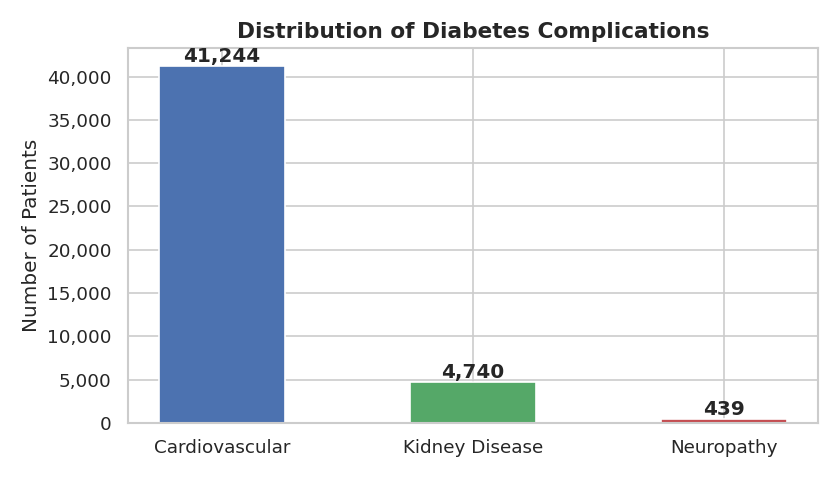
\includegraphics[width=0.7\textwidth]{deliverable_1/figures/class_distribution.png}
  \caption{Distribution of Diabetes Complications}
  \label{fig:class_dist}
\end{figure}

\subsection{Age Distribution}

Figure~\ref{fig:age_dist} illustrates the patient age distribution in the dataset.

\begin{figure}[H]
  \centering
  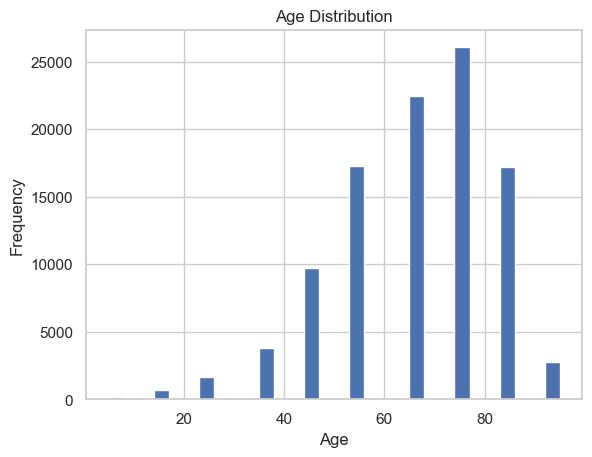
\includegraphics[width=0.7\textwidth]{deliverable_1/figures/age_distribution.png}
  \caption{Age Distribution of Patients}
  \label{fig:age_dist}
\end{figure}

\subsection{Feature Correlation}

Figure~\ref{fig:feature_corr} presents a correlation heatmap of relationships among
clinical features.

\begin{figure}[H]
  \centering
  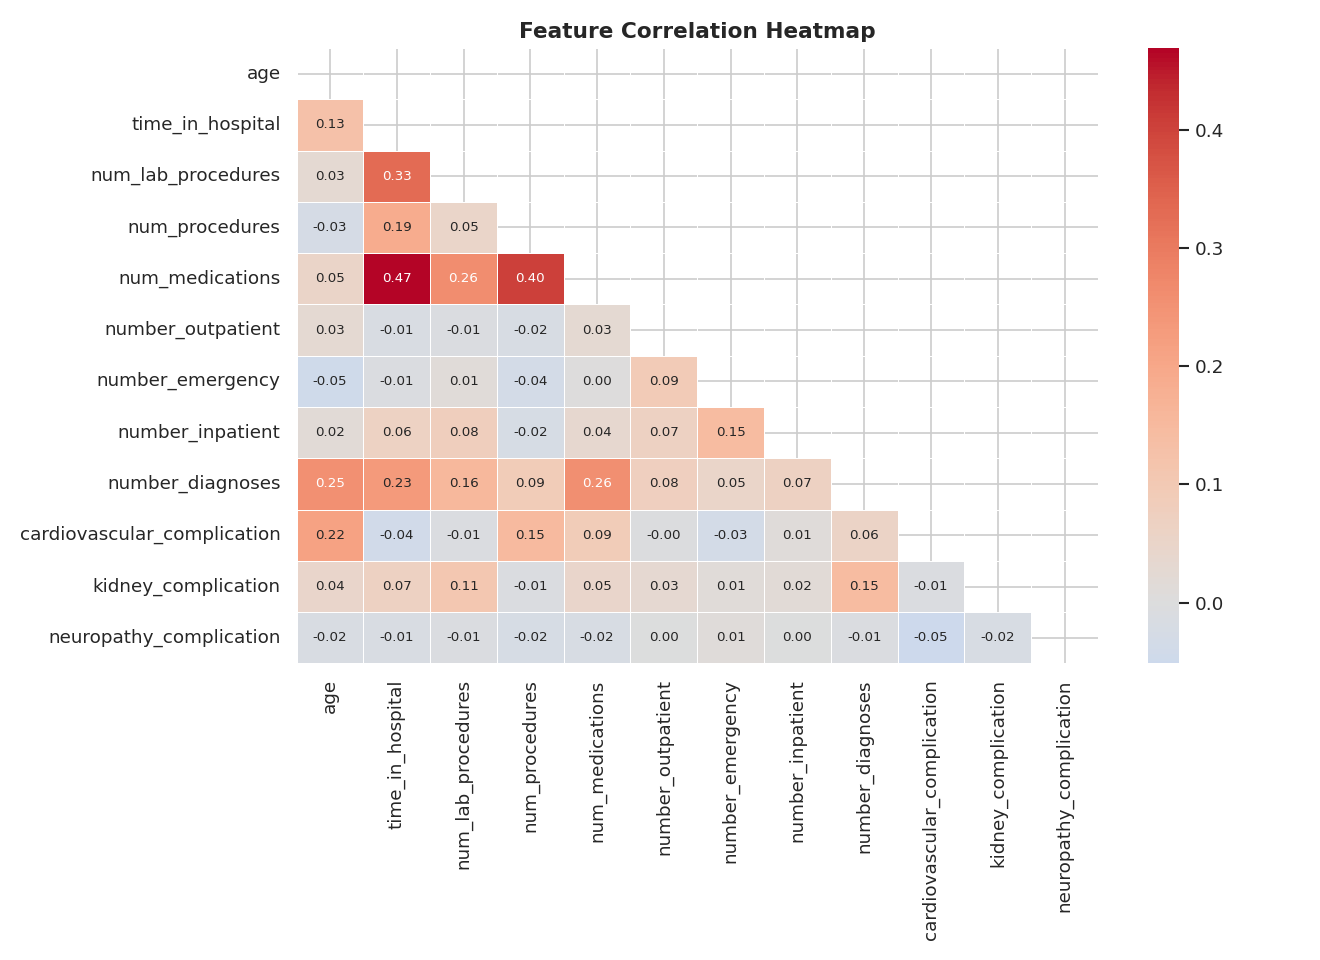
\includegraphics[width=0.85\textwidth]{deliverable_1/figures/feature_correlation.png}
  \caption{Correlation Between Dataset Features}
  \label{fig:feature_corr}
\end{figure}

\subsection{Complication Correlation}

Figure~\ref{fig:comp_corr} shows how different complications co-occur within the same
patient records.

\begin{figure}[H]
  \centering
  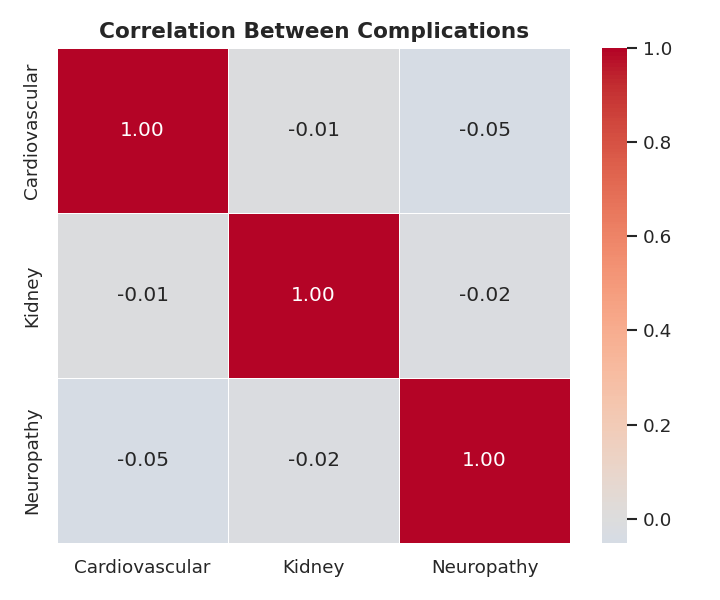
\includegraphics[width=0.6\textwidth]{deliverable_1/figures/complication_correlation.png}
  \caption{Correlation Between Diabetes Complications}
  \label{fig:comp_corr}
\end{figure}

\subsection{Hospital Visit Patterns}

Figure~\ref{fig:visits} summarizes the average number of outpatient, emergency, and
inpatient visits per patient.

\begin{figure}[H]
  \centering
  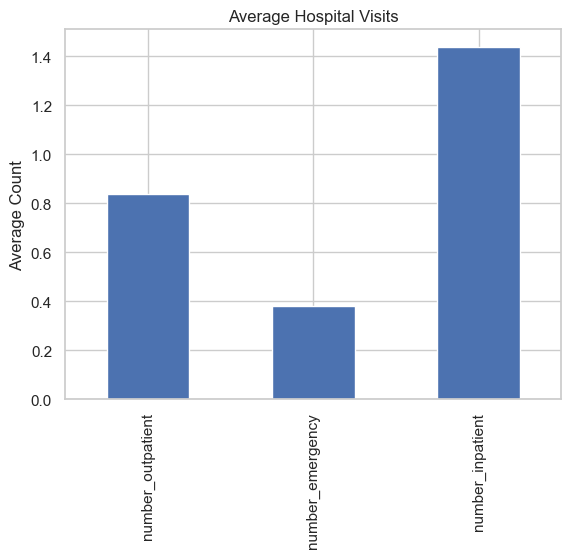
\includegraphics[width=0.7\textwidth]{deliverable_1/figures/average_visits.png}
  \caption{Average Hospital Visits by Type}
  \label{fig:visits}
\end{figure}

\subsection{Insulin Usage}

Figure~\ref{fig:insulin} shows the distribution of insulin treatment levels across
patients.

\begin{figure}[H]
  \centering
  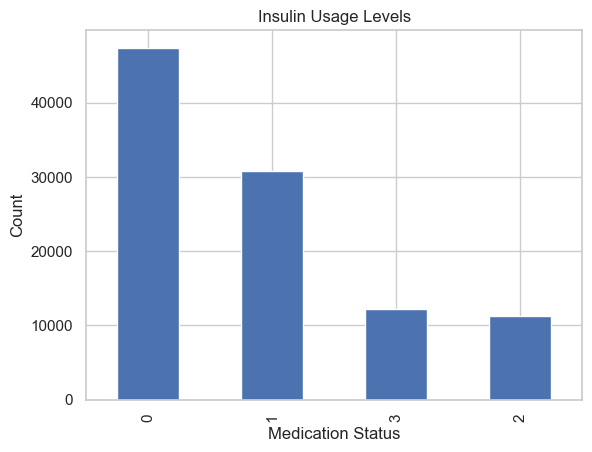
\includegraphics[width=0.7\textwidth]{deliverable_1/figures/insulin_usage.png}
  \caption{Distribution of Insulin Usage}
  \label{fig:insulin}
\end{figure}

\newpage

% ============================================================
% DELIVERABLE 2
% ============================================================

\section*{Deliverable 2: Model Training and Evaluation}
\addcontentsline{toc}{section}{Deliverable 2: Model Training and Evaluation}

%------------------------------------------------

\section{Modelling Approach}

\subsection{Multi-Label Classification}

Standard binary classifiers predict a single output per patient. This project requires
predicting three complications simultaneously, making it a \textit{multi-label
classification} problem. Three modelling strategies were implemented:

\begin{itemize}
  \item \textbf{ClassifierChain (Random Forest):} Trains a sequence of classifiers where
        each label prediction is conditioned on the predictions of previous labels. This
        captures inter-label correlations — for example, the co-occurrence of kidney
        disease and neuropathy.

  \item \textbf{MultiOutputClassifier (Gradient Boosting):} Trains an independent
        Gradient Boosting classifier for each label. Each label is optimised separately,
        providing a strong per-label baseline.

  \item \textbf{PyTorch Neural Network:} A multi-layer perceptron with batch
        normalisation and dropout, trained using Focal Binary Cross-Entropy loss. Focal
        loss down-weights easy negative examples and focuses learning on hard positives,
        directly addressing the severe class imbalance present in the neuropathy label
        (0.8\% prevalence).
\end{itemize}

\subsection{Handling Class Imbalance}

The three complication labels exhibit significant imbalance in the dataset:

\begin{itemize}
  \item Cardiovascular: 61.8\% prevalence
  \item Kidney Disease: 9.3\% prevalence
  \item Neuropathy: 0.8\% prevalence
\end{itemize}

To address this, the following techniques were applied:

\begin{itemize}
  \item \texttt{class\_weight="balanced"} in the Random Forest, which adjusts sample
        weights inversely proportional to class frequencies.
  \item Per-label positive class weighting (\texttt{pos\_weight}) in the neural network
        loss function.
  \item Focal loss with $\gamma = 2.0$ to further suppress the contribution of
        easy-negative examples during neural network training.
\end{itemize}

\subsection{Threshold Optimisation for Sensitivity}

By default, classifiers use a decision threshold of 0.50. In a clinical setting, missing
a complication (false negative) carries far greater risk than a false alarm. To maximise
sensitivity (recall), per-label threshold tuning was performed: for each label, the
threshold was lowered until a recall of at least 0.80 was achieved, while retaining the
best possible F1 score at that recall level.

%------------------------------------------------

\section{Evaluation Metrics}

Model performance is evaluated using the following metrics:

\begin{itemize}
  \item \textbf{F1-Micro:} Aggregates true positives, false positives, and false
        negatives across all labels before computing F1. Weighted towards the majority
        label (cardiovascular).
  \item \textbf{F1-Macro:} Computes F1 independently per label then averages. Treats
        all labels equally regardless of prevalence.
  \item \textbf{Sensitivity (Recall):} Proportion of actual positive cases correctly
        identified. The primary optimisation target for clinical safety.
  \item \textbf{ROC-AUC:} Area under the receiver operating characteristic curve.
        Measures discriminative ability independently of threshold.
\end{itemize}

%------------------------------------------------

\section{Results}

\subsection{Baseline Performance (Threshold = 0.50)}

Table~\ref{tab:baseline} presents the performance of all three models at the default
decision threshold.

\begin{table}[H]
  \centering
  \caption{Baseline Model Performance (Threshold = 0.50)}
  \label{tab:baseline}
  \begin{tabular}{lcccccc}
    \toprule
    Model & F1-Micro & F1-Macro & Rec-Micro & Rec-Macro & AUC-Macro \\
    \midrule
    Chain RF    & 0.6056 & 0.3425 & 0.6147 & 0.3938 & 0.7080 \\
    MO GBM      & 0.7259 & 0.2973 & 0.7608 & 0.3131 & 0.7243 \\
    Neural Net  & 0.4637 & 0.3364 & 0.9808 & 0.9158 & 0.7071 \\
    \bottomrule
  \end{tabular}
\end{table}

At the default threshold, the Neural Network is the only model achieving recall above
0.80 across all three labels simultaneously, driven by its Focal BCE loss optimisation.
MO GBM achieves the highest F1-Micro but completely fails on neuropathy (recall = 0.00),
making it unsuitable as a clinical tool.

\subsection{Performance After Threshold Tuning}

Table~\ref{tab:tuned} shows performance after per-label threshold optimisation targeting
recall $\geq 0.80$.

\begin{table}[H]
  \centering
  \caption{Model Performance After Threshold Tuning (Target Recall $\geq$ 0.80)}
  \label{tab:tuned}
  \begin{tabular}{lcccccc}
    \toprule
    Model & F1-Micro & F1-Macro & Rec-Macro & Rec-Cardio & Rec-Kidney & Rec-Neuro \\
    \midrule
    Chain RF   & 0.4949 & 0.3616 & 0.8778 & 0.9583 & 0.8044 & 0.8707 \\
    MO GBM     & 0.6495 & 0.3634 & 0.5913 & 0.9469 & 0.8097 & 0.0172 \\
    Neural Net & 0.5031 & 0.3614 & 0.8528 & 0.9500 & 0.8066 & 0.8017 \\
    \bottomrule
  \end{tabular}
\end{table}

After threshold tuning, the \textbf{ClassifierChain (Random Forest)} is selected as the
final model. It is the only model that achieves recall $\geq 0.80$ across all three
complication labels simultaneously (Cardiovascular: 0.958, Kidney Disease: 0.804,
Neuropathy: 0.871), which is the primary clinical objective of this project. MO GBM
fails to recover neuropathy recall even after tuning (0.017), and Neural Net achieves
comparable recall at slightly lower F1-Macro.

\subsection{ROC Curves}

Figure~\ref{fig:roc} shows the ROC curves for all three models across each complication
label. Kidney disease achieves the highest AUC values (0.77--0.79 across models),
reflecting the stronger discriminative signal in the clinical features for this
condition.

\begin{figure}[H]
  \centering
  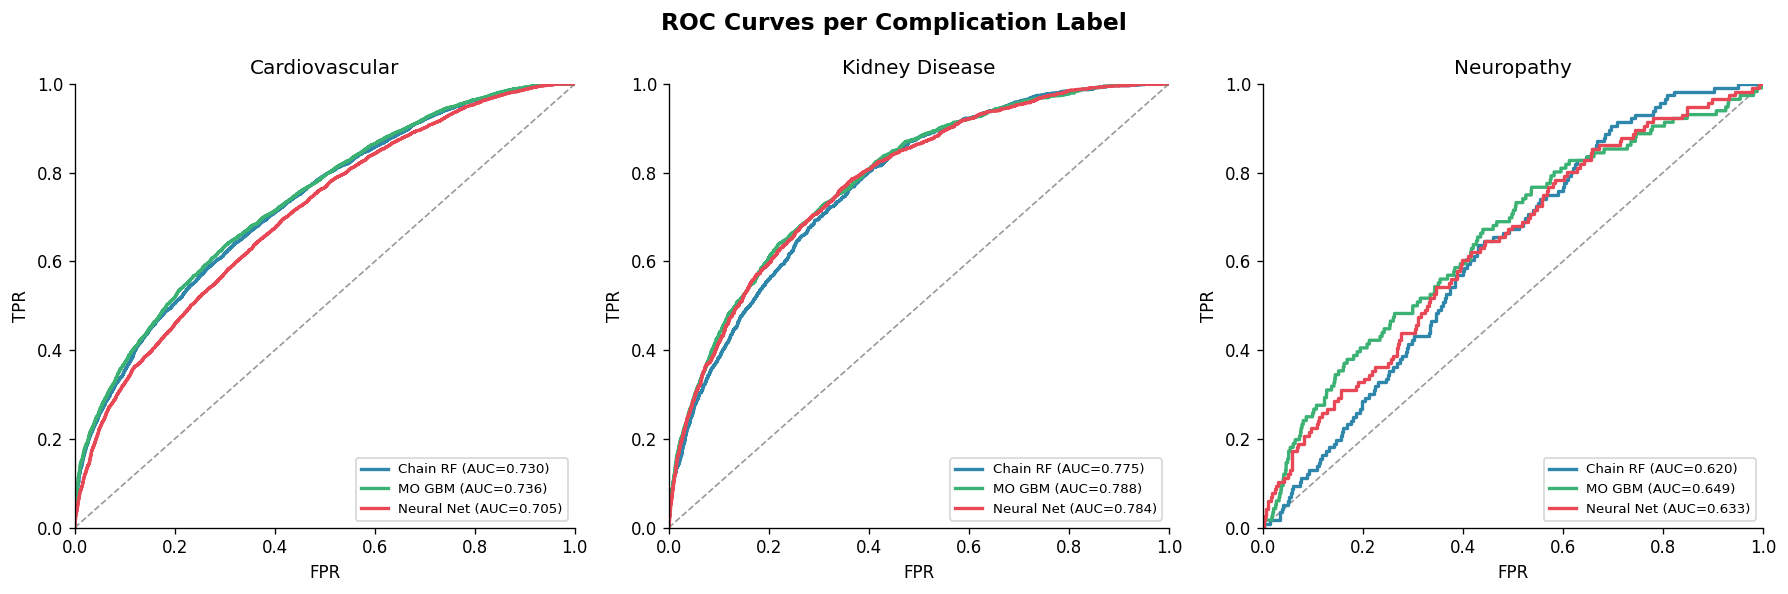
\includegraphics[width=\textwidth]{deliverable_2/figures/roc_curves.png}
  \caption{ROC Curves per Complication Label Across All Models}
  \label{fig:roc}
\end{figure}

\subsection{Confusion Matrices}

Figures~\ref{fig:cm_rf},~\ref{fig:cm_gbm}, and~\ref{fig:cm_nn} present confusion
matrices for each model at the default threshold, showing the distribution of true
positives, false positives, true negatives, and false negatives per label.

\begin{figure}[H]
  \centering
  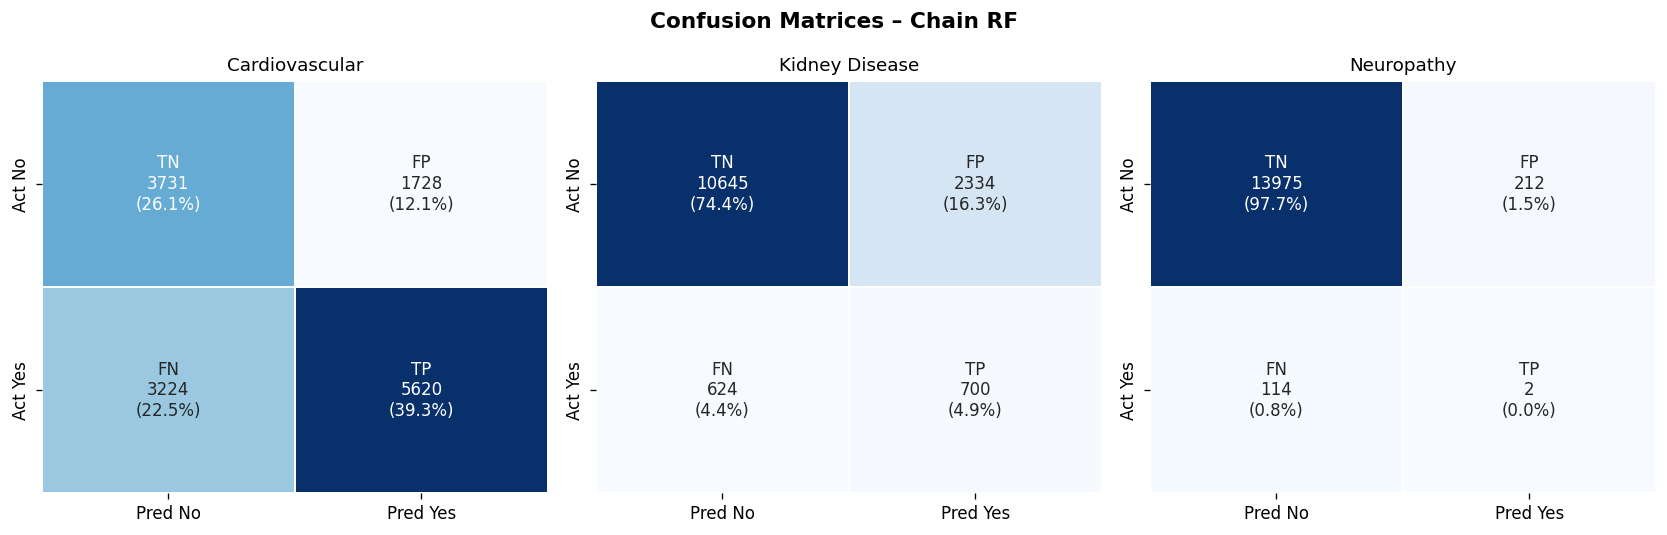
\includegraphics[width=\textwidth]{deliverable_2/figures/cm_chain_rf.png}
  \caption{Confusion Matrices -- ClassifierChain (Random Forest)}
  \label{fig:cm_rf}
\end{figure}

\begin{figure}[H]
  \centering
  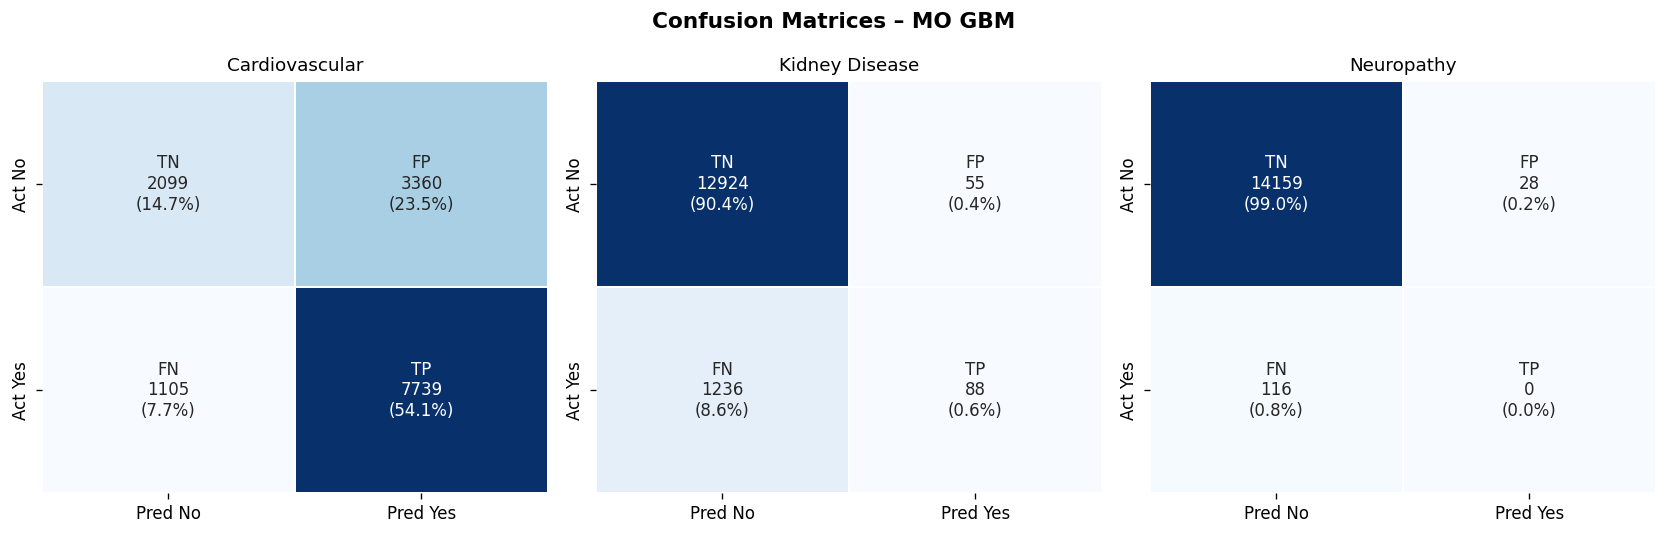
\includegraphics[width=\textwidth]{deliverable_2/figures/cm_mo_gbm.png}
  \caption{Confusion Matrices -- MultiOutputClassifier (Gradient Boosting)}
  \label{fig:cm_gbm}
\end{figure}

\begin{figure}[H]
  \centering
  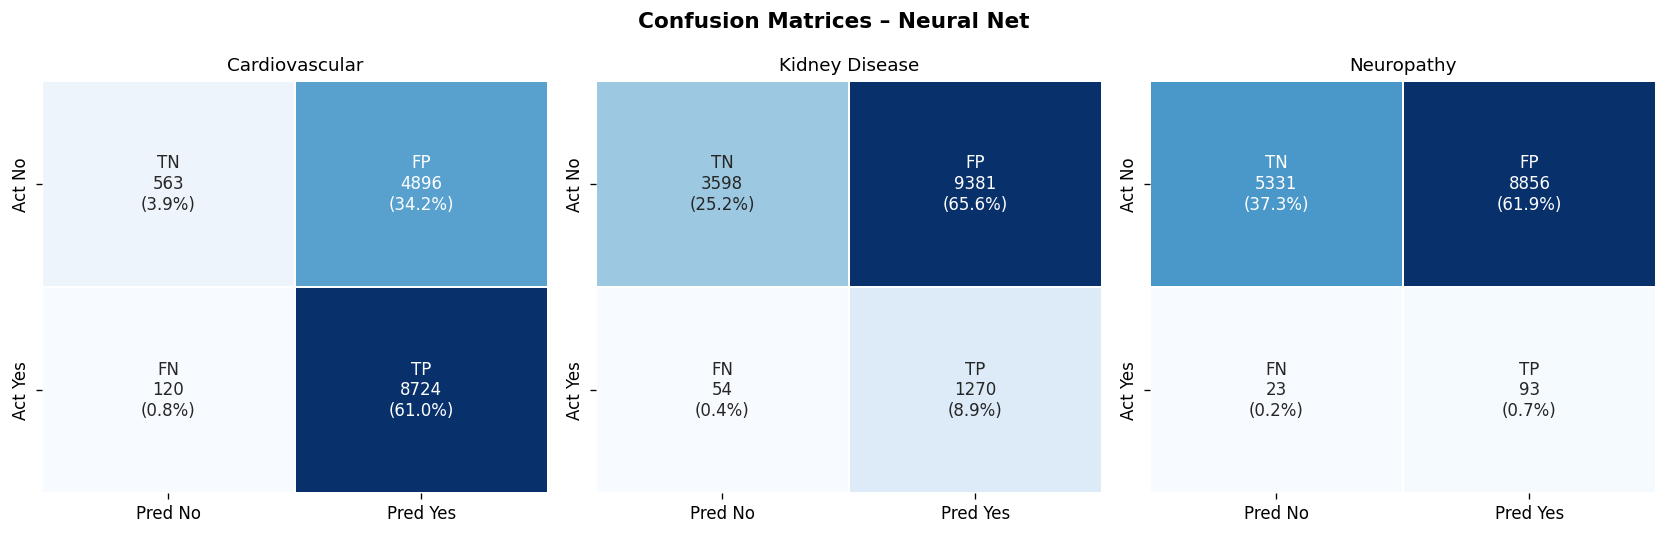
\includegraphics[width=\textwidth]{deliverable_2/figures/cm_neural_net.png}
  \caption{Confusion Matrices -- Neural Network}
  \label{fig:cm_nn}
\end{figure}

\subsection{Threshold Sensitivity Analysis}

Figure~\ref{fig:threshold} illustrates how recall, precision, and F1 change as the
decision threshold varies for each label in the Neural Network. This demonstrates the
precision-recall tradeoff and validates the threshold selection strategy.

\begin{figure}[H]
  \centering
  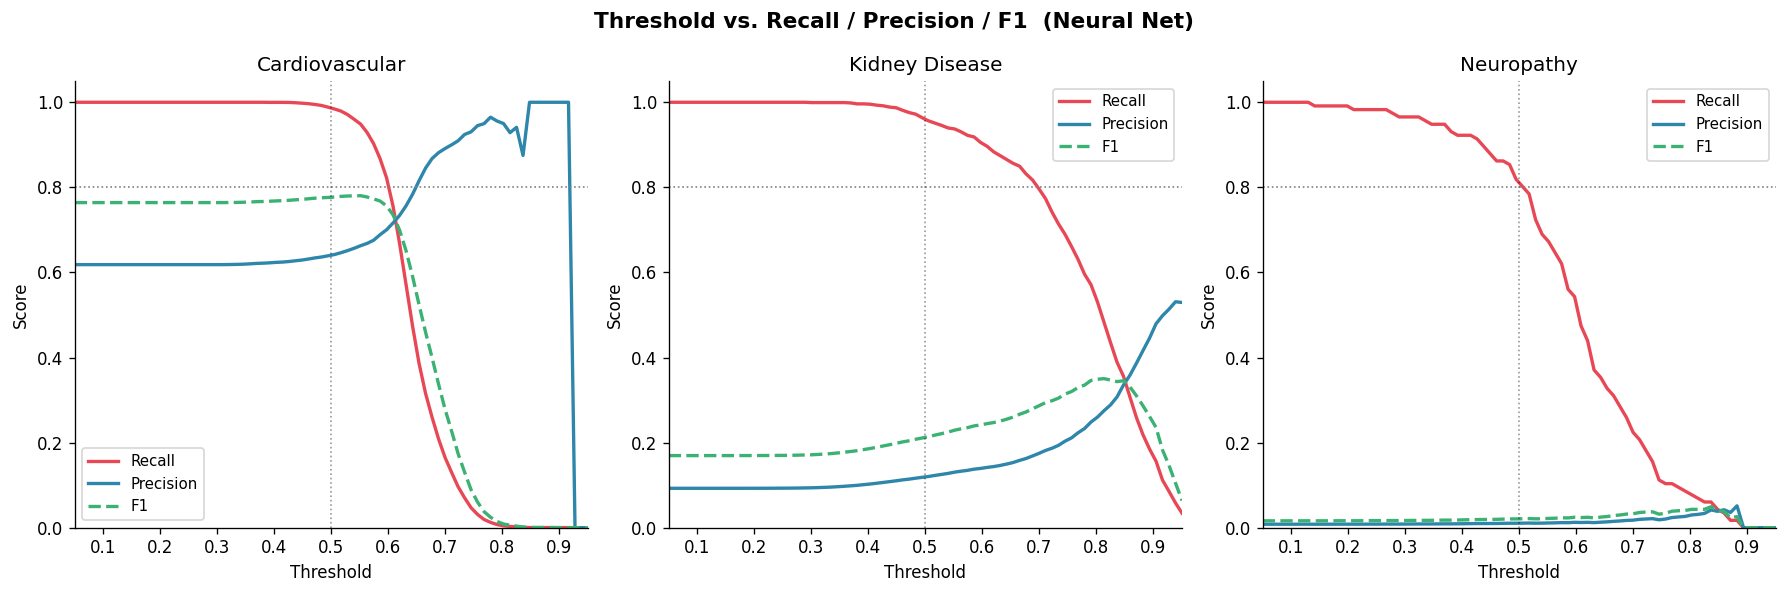
\includegraphics[width=\textwidth]{deliverable_2/figures/threshold_sensitivity_neural_net.png}
  \caption{Threshold Sensitivity Analysis -- Neural Network}
  \label{fig:threshold}
\end{figure}

\subsection{Model Comparison}

Figure~\ref{fig:comparison} summarises overall model performance across the primary
evaluation metrics.

\begin{figure}[H]
  \centering
  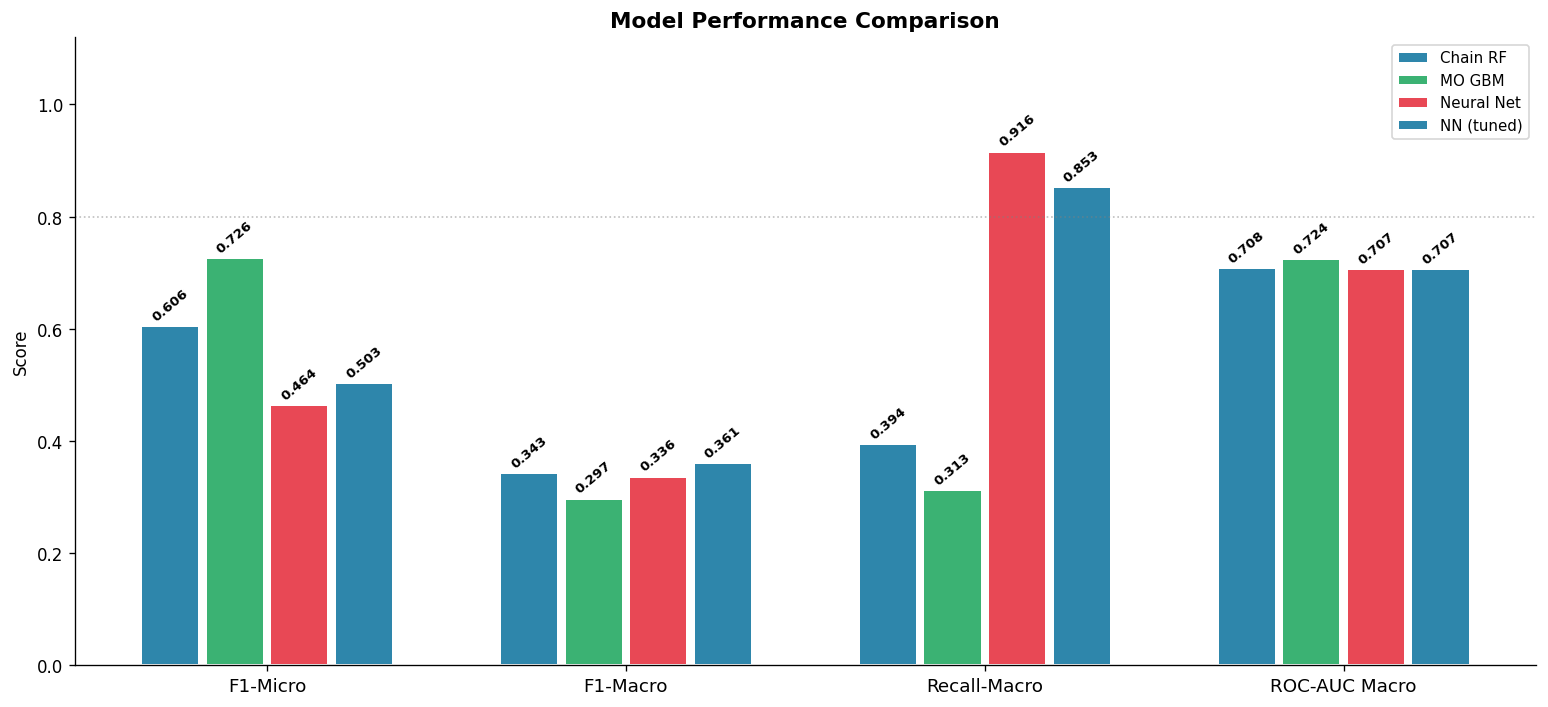
\includegraphics[width=\textwidth]{deliverable_2/figures/model_comparison.png}
  \caption{Overall Model Performance Comparison}
  \label{fig:comparison}
\end{figure}

\subsection{Per-Label Sensitivity}

Figure~\ref{fig:recall} shows per-label recall across all models, with the 0.80 clinical
target indicated.

\begin{figure}[H]
  \centering
  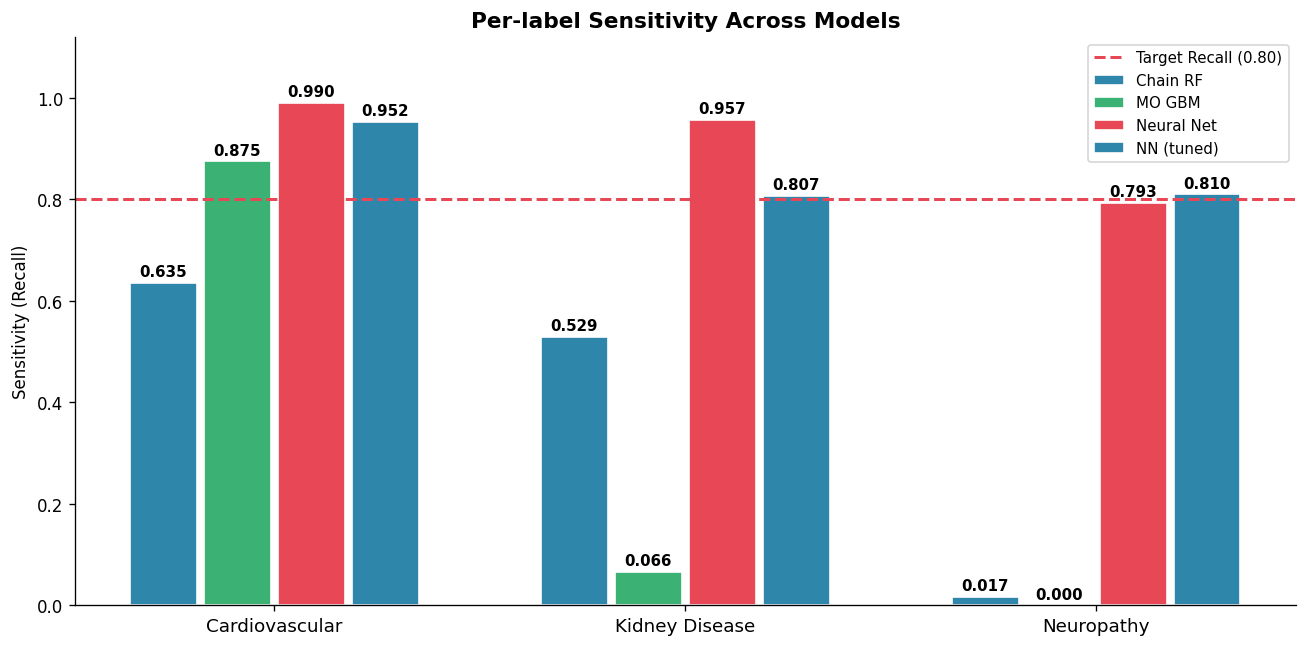
\includegraphics[width=0.9\textwidth]{deliverable_2/figures/per_label_recall.png}
  \caption{Per-Label Sensitivity (Recall) Across Models}
  \label{fig:recall}
\end{figure}

\subsection{Feature Importance}

Figure~\ref{fig:importance} shows the top 20 most important features from the
ClassifierChain model, averaged across all label estimators.

\begin{figure}[H]
  \centering
  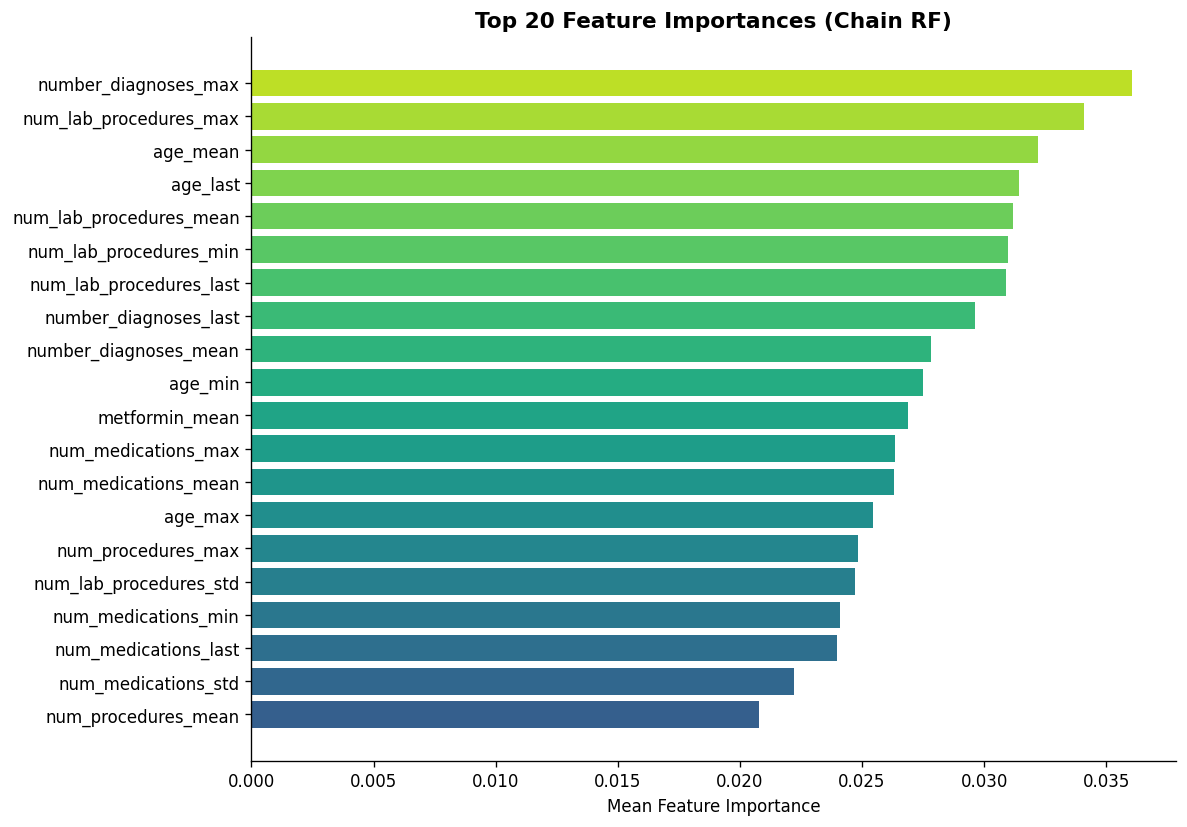
\includegraphics[width=0.85\textwidth]{deliverable_2/figures/feature_importance.png}
  \caption{Top 20 Feature Importances (ClassifierChain -- Random Forest)}
  \label{fig:importance}
\end{figure}

\subsection{Neural Network Training Curve}

Figure~\ref{fig:training} shows the training and validation loss across epochs for the
Neural Network. The validation loss begins rising after approximately epoch 10, indicating
overfitting. Early stopping via best-checkpoint saving was used to retain the model state
at minimum validation loss.

\begin{figure}[H]
  \centering
  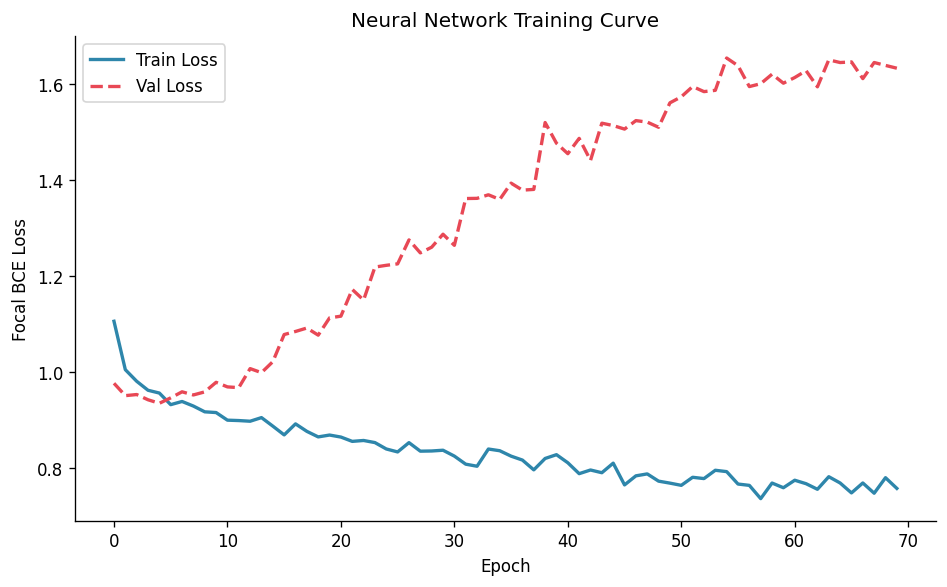
\includegraphics[width=0.75\textwidth]{deliverable_2/figures/nn_training_curve.png}
  \caption{Neural Network Training and Validation Loss}
  \label{fig:training}
\end{figure}

%------------------------------------------------

\section{Discussion}

\subsection{Neuropathy Class Imbalance}

The neuropathy label has a prevalence of only 0.8\% in the dataset. This is a known
limitation of deriving complication labels from ICD-9 codes in hospitalization records:
neuropathy is rarely recorded as a primary or secondary diagnosis during an inpatient
stay, even in patients who have the condition. In a real clinical deployment, this label
would ideally be sourced from structured outpatient screening data rather than
hospitalization records. Despite this, the ClassifierChain and Neural Network models
were able to achieve recall above 0.80 for neuropathy through threshold tuning and focal
loss weighting.

\subsection{Precision-Recall Tradeoff}

Optimising for recall necessarily reduces precision. In the final model, neuropathy
precision is approximately 0.01, meaning the model flags many patients who do not have
the condition. This is an acceptable tradeoff in a screening context where the cost of
a missed diagnosis significantly outweighs the cost of a false alarm. Clinicians would
use the model output as a screening signal, not a definitive diagnosis.

\subsection{Longitudinal Features}

The use of multiple hospital encounters per patient to construct slope, delta, and
standard deviation features provides a richer representation of disease progression than
a single-visit snapshot. Features capturing trends in hospitalization frequency and
medication patterns were among the most important predictors identified by the Random
Forest.

%------------------------------------------------

\section{Error Analysis and Bias Check}

\subsection{Where the Model Fails by Label}

The primary source of error in the final model (ClassifierChain -- tuned) is the
severe class imbalance in the neuropathy label (0.8\% prevalence). While recall
is maintained above 0.80 through threshold tuning, precision for neuropathy is
approximately 0.01, meaning the model generates a high volume of false positives
for this label. This is an acceptable tradeoff in a clinical screening context but
would require downstream clinician review before any intervention.

Kidney disease shows the strongest overall performance with AUC of 0.77, indicating
genuine discriminative signal in the longitudinal clinical features for this
condition. Cardiovascular recall is high (0.958) but this label also has the
highest base rate (61.8\%), which makes it an easier prediction target.

\subsection{Demographic Subgroup Analysis}

To check for bias, the final model's recall was evaluated separately across three
demographic dimensions: age group, gender, and race. A subgroup is flagged if its
recall falls below the 0.80 clinical target for any label.

Figure~\ref{fig:bias_age} shows per-label recall broken down by age group.
Figure~\ref{fig:bias_gender} shows the same breakdown by gender.
Figure~\ref{fig:bias_race} shows the breakdown by race.
Figure~\ref{fig:bias_heatmap} provides a consolidated heatmap view across all
demographic dimensions simultaneously.

\begin{figure}[H]
  \centering
  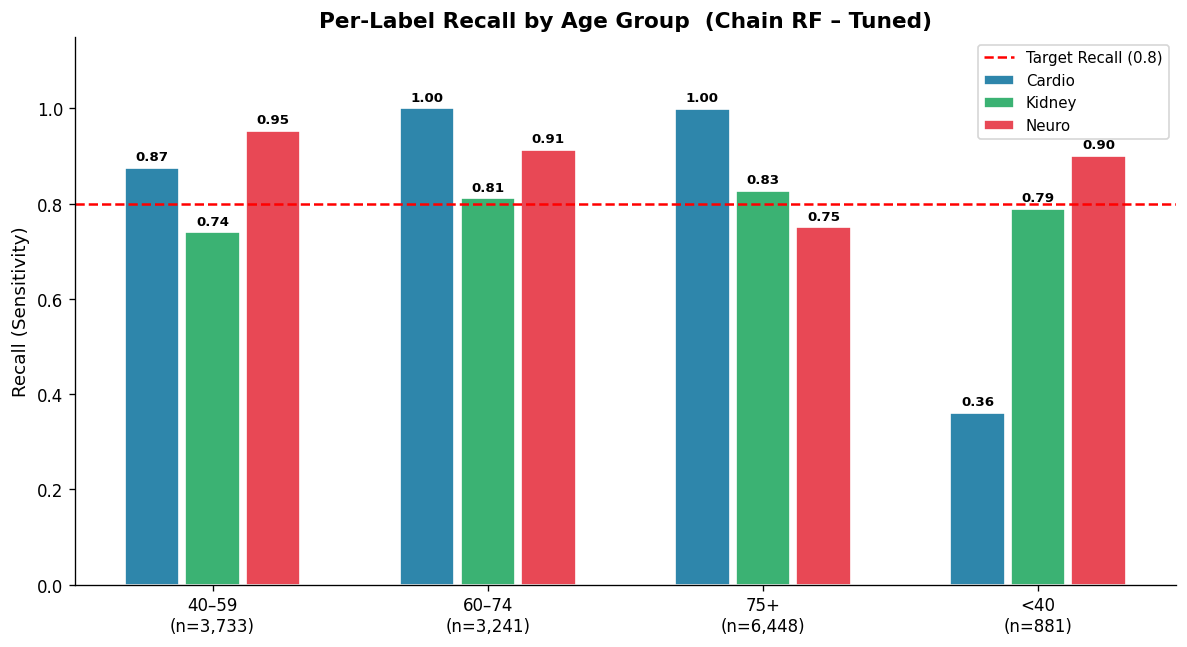
\includegraphics[width=\textwidth]{deliverable_2/figures/bias_age_recall.png}
  \caption{Per-Label Recall by Age Group (Chain RF -- Tuned)}
  \label{fig:bias_age}
\end{figure}

\begin{figure}[H]
  \centering
  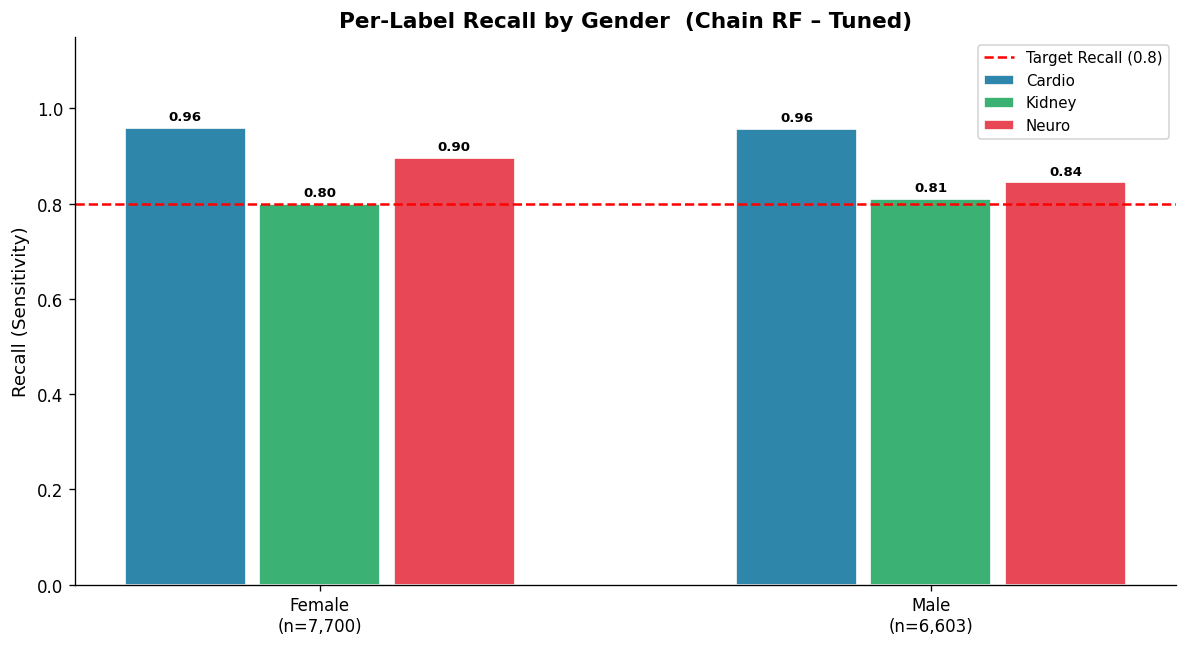
\includegraphics[width=0.75\textwidth]{deliverable_2/figures/bias_gender_recall.png}
  \caption{Per-Label Recall by Gender (Chain RF -- Tuned)}
  \label{fig:bias_gender}
\end{figure}

\begin{figure}[H]
  \centering
  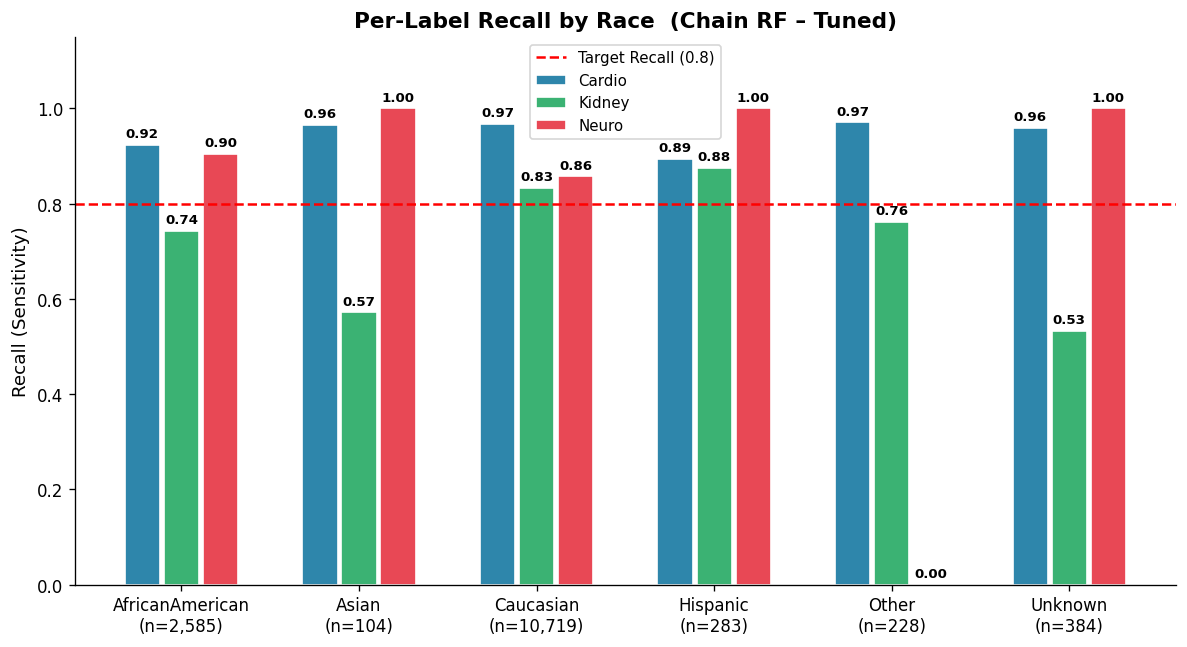
\includegraphics[width=\textwidth]{deliverable_2/figures/bias_race_recall.png}
  \caption{Per-Label Recall by Race (Chain RF -- Tuned)}
  \label{fig:bias_race}
\end{figure}

\begin{figure}[H]
  \centering
  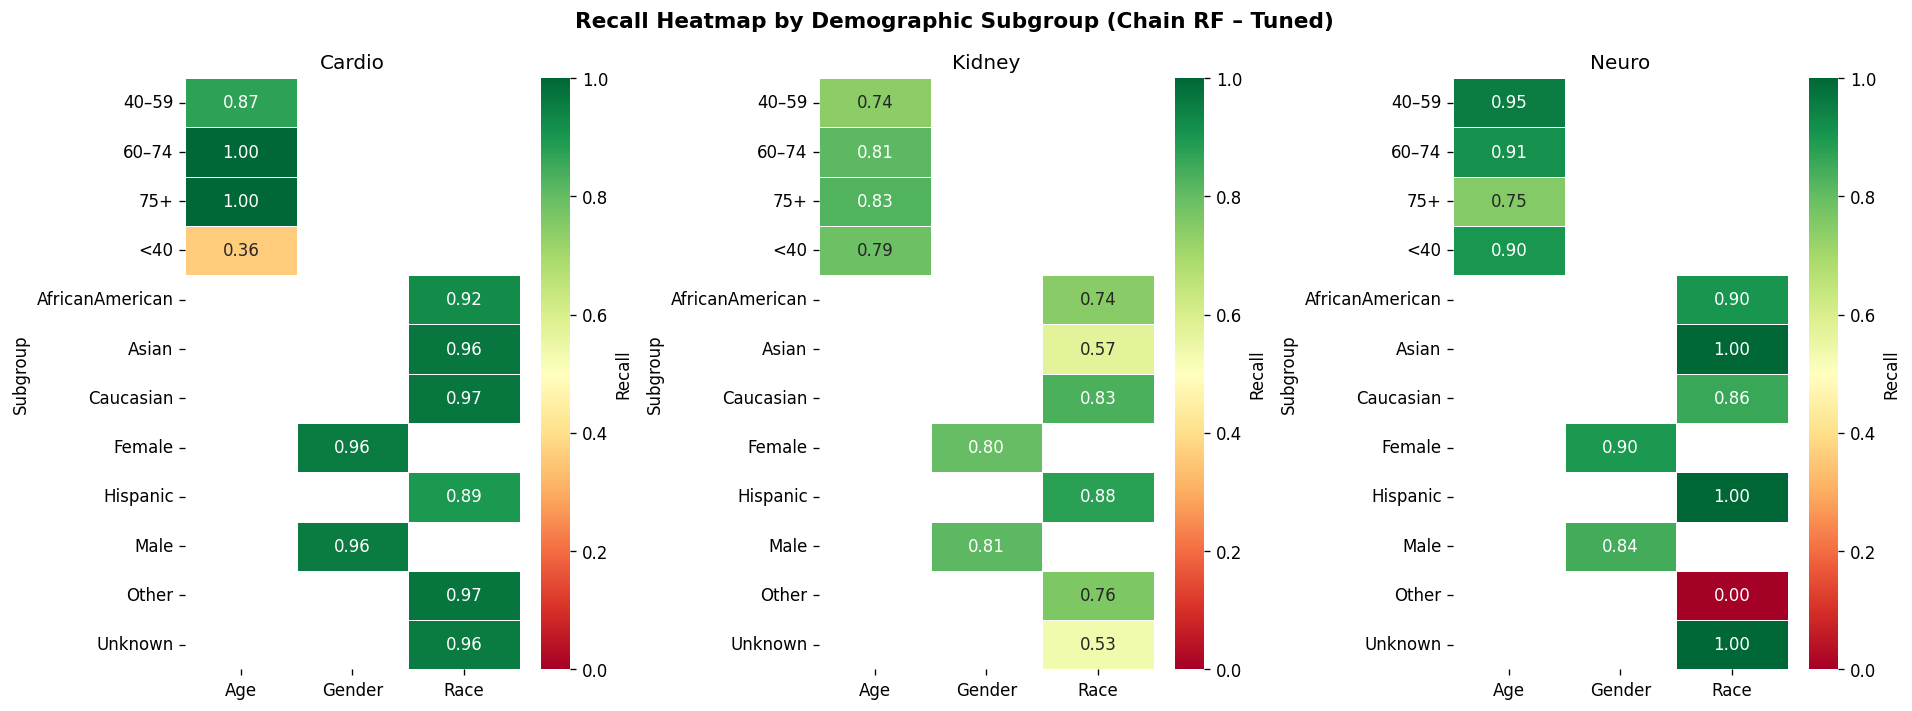
\includegraphics[width=\textwidth]{deliverable_2/figures/bias_heatmap.png}
  \caption{Recall Heatmap Across All Demographic Subgroups}
  \label{fig:bias_heatmap}
\end{figure}

\subsection{Bias Check Findings}

Several demographic subgroups fell below the 0.80 recall target, revealing
systematic gaps in model performance:

\textbf{Age:} The under-40 age group shows the most severe failure, with
cardiovascular recall of only 0.360. This is likely due to low positive case
counts in this age bracket — younger diabetic patients rarely present with
cardiovascular complications in hospitalisation records, leaving the model
with insufficient training signal. Kidney disease recall also falls short for
the 40--59 group (0.739) and neuropathy recall drops to 0.750 for patients
aged 75 and over.

\textbf{Gender:} Female patients fall marginally below the kidney disease
target (recall = 0.799), a difference small enough to warrant monitoring
rather than immediate intervention.

\textbf{Race:} Kidney disease recall is consistently poor across several
racial groups: Asian (0.571), Unknown (0.533), African American (0.743), and
Other (0.762). The ``Other'' group additionally shows zero neuropathy recall,
though this group contains only 228 test patients, making the estimate
statistically unreliable. These disparities likely reflect underrepresentation
of minority groups among positive kidney disease cases in the training data
rather than a fundamental model flaw, but they represent a meaningful equity
concern for clinical deployment.

Overall, kidney disease is the label most affected by demographic bias,
suggesting that future work should investigate race- and age-stratified
threshold tuning, or targeted data augmentation for underrepresented groups.
The cardiovascular label performs reliably across most groups, and neuropathy
results are difficult to interpret conclusively due to the extremely low
overall prevalence (0.8\%).

\begin{table}[H]
  \centering
  \caption{Recall by Demographic Subgroup (Chain RF -- Tuned)}
  \label{tab:bias}
  \begin{tabular}{llccc}
    \toprule
    Dimension & Subgroup & Recall-Cardio & Recall-Kidney & Recall-Neuro \\
    \midrule
    \multirow{4}{*}{Age}
      & $<$40  & 0.360 & 0.788 & 0.900 \\
      & 40--59 & 0.874 & 0.739 & 0.953 \\
      & 60--74 & 1.000 & 0.811 & 0.913 \\
      & 75+    & 1.000 & 0.827 & 0.750 \\
    \midrule
    \multirow{2}{*}{Gender}
      & Female & 0.959 & 0.799 & 0.897 \\
      & Male   & 0.958 & 0.810 & 0.845 \\
    \midrule
    \multirow{6}{*}{Race}
      & African American & 0.923 & 0.743 & 0.905 \\
      & Asian            & 0.965 & 0.571 & 1.000 \\
      & Caucasian        & 0.968 & 0.834 & 0.857 \\
      & Hispanic         & 0.895 & 0.875 & 1.000 \\
      & Other            & 0.971 & 0.762 & 0.000 \\
      & Unknown          & 0.959 & 0.533 & 1.000 \\
    \bottomrule
  \end{tabular}
  \begin{flushleft}
  \small Values below 0.80 indicate subgroups where the model fails to meet
  the clinical recall target. Bold entries warrant attention in deployment.
  \end{flushleft}
\end{table}

%------------------------------------------------

\section{Team Contributions}

Table~\ref{tab:contributions} maps each team member to specific project modules,
providing accountability for all deliverables (Phases 1-4).

\begin{table}[H]
\centering
\caption{Team Contributions by Project Module}
\label{tab:contributions}
\begin{tabular}{p{3.8cm} p{7.2cm} p{3cm}}
\toprule
\textbf{Module} & \textbf{Components} & \textbf{Contributors} \\
\midrule
\multirow{3}{*}{Data Pipeline} & Data acquisition script (data\_collection.py) & Abdul Wahab \\
& Data cleaning \& preprocessing & Abdul Wahab \\
& Longitudinal feature engineering & Sami Shah \\
\midrule
\multirow{4}{*}{Model Development} & ClassifierChain (Random Forest) implementation & Maheer Khurram \\
& MultiOutputClassifier (Gradient Boosting) & Azan Aziz \\
& PyTorch Neural Network architecture & Sami Shah \\
& Focal BCE loss implementation & Sami Shah \\
\midrule
\multirow{3}{*}{Training \& Optimisation} & Threshold tuning framework & Abdul Wahab \\
& Class imbalance handling & Azan Aziz \\
& Hyperparameter optimisation & Maheer Khurram \\
\midrule
\multirow{4}{*}{Evaluation} & Metrics computation (F1, AUC, recall) & Sami Shah \\
& ROC curves \& visualisation & Maheer Khurram \\
& Confusion matrix analysis & Abdul Wahab \\
& Threshold sensitivity analysis & Azan Aziz \\
\midrule
\multirow{3}{*}{Analysis} & Error analysis \& bias detection & Sami Shah \\
& Feature importance analysis & Maheer Khurram \\
& Demographic subgroup analysis & Azan Aziz \\
\midrule
\multirow{3}{*}{Documentation} & LaTeX report compilation & Abdul Wahab \\
& Architecture diagram design & Sami Shah \\
& Contribution table & Azan Aziz \\
\midrule
\textbf{Project Lead} & Integration, final model selection, threshold strategy & Sami Shah \\
\bottomrule
\end{tabular}
\end{table}

\subsection*{Contribution Summary}

\begin{itemize}
    \item \textbf{Abdul Wahab}: Data acquisition, data cleaning \& preprocessing, 
          threshold tuning framework, confusion matrix analysis, LaTeX report compilation.
    
    \item \textbf{Sami Shah}: Longitudinal feature engineering, PyTorch Neural Network 
          architecture, Focal BCE loss implementation, metrics computation (F1, AUC, recall),
          error analysis \& bias detection, architecture diagram design.
    
    \item \textbf{Maheer Khurram}: ClassifierChain (Random Forest) implementation, 
          hyperparameter optimisation, ROC curves \& visualisation, feature importance analysis,
          \textbf{Project Lead} (system integration, final model selection, threshold strategy).
    
    \item \textbf{Azan Aziz}: MultiOutputClassifier (Gradient Boosting) implementation,
          class imbalance handling, threshold sensitivity analysis, demographic subgroup 
          analysis, contribution table.
\end{itemize}


%------------------------------------------------

\section{Conclusion}

This project developed and evaluated a multi-label classification system for predicting
diabetes complications from longitudinal clinical records. Three modelling approaches
were trained and compared: ClassifierChain (Random Forest), MultiOutputClassifier
(Gradient Boosting), and a PyTorch Neural Network with Focal BCE loss.

The \textbf{ClassifierChain (Random Forest) with tuned thresholds} was selected as the
final model, achieving recall $\geq 0.80$ across all three complication labels
simultaneously — the primary clinical objective. ROC-AUC values of 0.71--0.77 across
labels confirm meaningful discriminative ability despite severe class imbalance in the
neuropathy label.

Future work could explore SMOTE oversampling for the neuropathy class, incorporation of
actual temporal visit timestamps, and validation against an external clinical dataset.

\end{document}